\documentclass{article} % For LaTeX2e
\usepackage{nips15submit_e,times}
\usepackage{hyperref}
\usepackage{url}
\usepackage{enumerate}
\usepackage{graphicx} 
%\documentstyle[nips14submit_09,times,art10]{article} % For LaTeX 2.09


\title{Report - Autonomous Driving: Object Detection}


\author{
Zhen Li \\
Department of Computer Science\\
University of Toronto\\
Toronto, ON, M5S 2E4 \\
\href{mailto:zhen@cs.toronto.edu}{\texttt{zhen@cs.toronto.edu}}
\And
Zhicong Lu \\
Department of Computer Science\\
University of Toronto\\
Toronto, ON, M5S 2E4 \\
\href{mailto:luzhc@cs.toronto.edu}{\texttt{luzhc@cs.toronto.edu}}
}

% The \author macro works with any number of authors. There are two commands
% used to separate the names and addresses of multiple authors: \And and \AND.
%
% Using \And between authors leaves it to \LaTeX{} to determine where to break
% the lines. Using \AND forces a linebreak at that point. So, if \LaTeX{}
% puts 3 of 4 authors names on the first line, and the last on the second
% line, try using \AND instead of \And before the third author name.

\newcommand{\fix}{\marginpar{FIX}}
\newcommand{\new}{\marginpar{NEW}}

%\nipsfinalcopy % Uncomment for camera-ready version

\begin{document}


\maketitle

\iffalse
\begin{abstract}
TODO: The abstract paragraph should be indented 1/2~inch (3~picas) on both left and
right-hand margins. Use 10~point type, with a vertical spacing of 11~points.
The word \textbf{Abstract} must be centered, bold, and in point size 12. Two
line spaces precede the abstract. The abstract must be limited to one
paragraph.
\end{abstract}
\fi

\section{Introduction}

Autonomous driving is one of the most challenging topic in Computer Vision as well as Machine Learning. The goal of this project is to detect the cars and pedestrians in the given images, locating the 2D bounding boxes of the objects correctly. Such detection techniques would make vision-based autonomous driving systems more robust and accurate, hence increasing the possibility of adopting them in the real life. 

It is hard to apply classical machine learning techniques on this topic directly. For example, we have learnt several object recognition algorithms which perform very well on MNIST \cite{lecun1998gradient} Database. However, the real road image has more occlution,  

The basic idea of this project came from The KITTI Vision Benchmark Suite \cite{Geiger2012CVPR} 

In this project, we focus on the performance of SVM, CNN, and boosting techniques as well as their differences. Our code is available on GitHub\footnote{https://github.com/CommanderLee/ObjectDetection}.

[old]The basic idea of this project came from The KITTI Vision Benchmark Suite [2]. According to the website, an overlap of 70\% is required for a detection of a car, while an overlap of 50\% is required for the pedestrians.

[old]To achieve our goals, we will download the left color images of object, camera calibration and training
labels data from \texttt{http://www.cvlibs.net/datasets/kitti/eval\_object.php}, as well as the development kit, upon which we will train the model and evaluate our methods. The labeled training data will be splitted into training, validation, and testing, which takes 60\%, 10\% and 30\% respectively. Besides KITTI, we would also use some other datasets to test our methods, especially on pedestrain detection, including Caltech Pedestrian Detection Benchmark[7] and Daimler Pedestrian Segmentation Benchmark Dataset[1].

[old]Inspired by the ranking of different methods on the KITTI website, we would try to implement those with very good performence and without using other sensor data, for the reason that such methods are more accessible and have better potential to be implemented even on mobile devices. We would try to improve the training model based on the findings of the state-of-the-art to come up with our own method, and evaluate the performance of it.We expect that our method can reach a high accuracy on the test set with an optimized speed. 

\section{Related work}

[old]Object detection, especially cars and pedestrains detecions for autonomous driving systems, has been a hot topic in computer vision for recent years. Convolutional Neural
Network(CNN or ConvNet)[6] is able to learn the features of the object and handle variations such as poses, viewpoints, and lightings, with high accuracy and high efficiency. However, it doesn't perform well when occlusion occurs, which is often the case in pedestrian and cyclists detection. 

[old]DeepParts[3] is a method to solve such problems, which consists of extensive strong part detectors to detect pedestrian by observing only a part
of a proposal. It can be trained on weakly labeled
data and performs very well on the task of pedestrain detection. 

[old]Recently, the Fully Convolutional Neural Network (FCN) based methods[5], with end-to-end approach of learning model parameters and image features, further improves the performance of object detection. DenseBox[4] is a unified end-to-end FCN that
directly predicts bounding boxes and object class confidences through all locations
and scales of an image with great accuracy and efficiancy. It also incorporates with landmark localization during multi-task learning and further improves
object detection accuracy. It has the best accuracy on car detection on KITTI by the time the proposal is finished. However, it has not been tested on the tasks of pedestrain or cyclists detection.

[old]Our method will be based on CNN and FCN, with some techniques to deal with occlusion and other issues. We will try to make it accurate on all of the three detection tasks. The performance of our methods will be compared with that of DeepParts and DenseBox.

In many tasks, since the number of images and windows to evaluate is huge, we often rely on a weak classifier to get proposals for the more expensive classifier. Selective Search \cite{van2011segmentation} is a successful algorithm, which emphasize recall to include all image fragments of potential relevance. 

\section{Methods}

\section{Experiments}

\subsection{Data set}

We use the KITTI data set for Object Detection \cite{Geiger2012CVPR}, which contains $7481$ color images with ground truth bounding box labels, including $28782$ cars and $4487$ pedestrians. We partition the data set to a training set contains $5237$ images($70\%$), and a testing set contains $2244$ images($30\%$). Then we run different algorithms on the data set and analyze the results.

\subsection{Pre-process: Selective Search}
\label{sec:preprocess}

First, we crop the cars and pedestrians from the images to generate the positive examples. We noticed that we have far more cars than pedestrians in the data set. To balance the difference, we multiply the pedestrian image set by adding a random bias to the color map (from $-20\%$ to $+20\%$) repeatedly. We also reverse the original image horizontally to make full use of the training set. Since the KITTI benchmark only evaluate objects larger than $25$ pixels (height), we ignore these small objects in the training set. After all of these augmenting and filtering strategies, we have $22576$ cars and $20960$ pedestrians as positive examples for training.

We use the Selective Search \cite{van2011segmentation} to generate the negative examples. We randomly select images from the training set, run Selective Search, and find out background segments, which have a $0\%$ to $30\%$ overlap with a positive example. We generate $20000$ negative examples for training. 

\subsection{Object Detection Procedure}

There are mainly two steps in our detection procedure: 
\begin{enumerate}[Step 1]
    \item Weak classifier: Generate proposals and save the bounding box.
    \item Strong classifier: Find out cars and pedestrians, and save the results.
\end{enumerate}

We use the Selective Search \cite{van2011segmentation} as the common weak classifier. For the strong classifier after it, we tried SVM, Regionlets, and CNN.

\subsection{Regionlets}

blablabla

\subsection{SVM}

\subsubsection{Training}

The SVM classifier is trained using the cropped positive examples with ground truth labels, and negative background segments generated by the Selective Search. Since SVM is a binary classifier, we trained 3 classifiers: (1) Car vs All, (2) Pedestrian vs All, and (3) Car vs Pedestrian. We use the \texttt{fitcsvm} function from the MATLAB toolbox.

\subsubsection{Validation}

We use the k-fold ($k=7$) cross validation to evaluate our model, as required by the project guide ($60\%$ training, $10\%$ validation, and $30\%$ testing). According to our description in Section \ref{sec:preprocess}, we multiply the data set by changing the contrast and brightness of the images, as well as reversing the images horizontally. Then we can compare the cross loss before and after the multiplication, using the \texttt{crossval} function from the MATLAB toolbox.

\begin{figure}[htb]
\begin{center}
%\framebox[4.0in]{crossloss.eps}
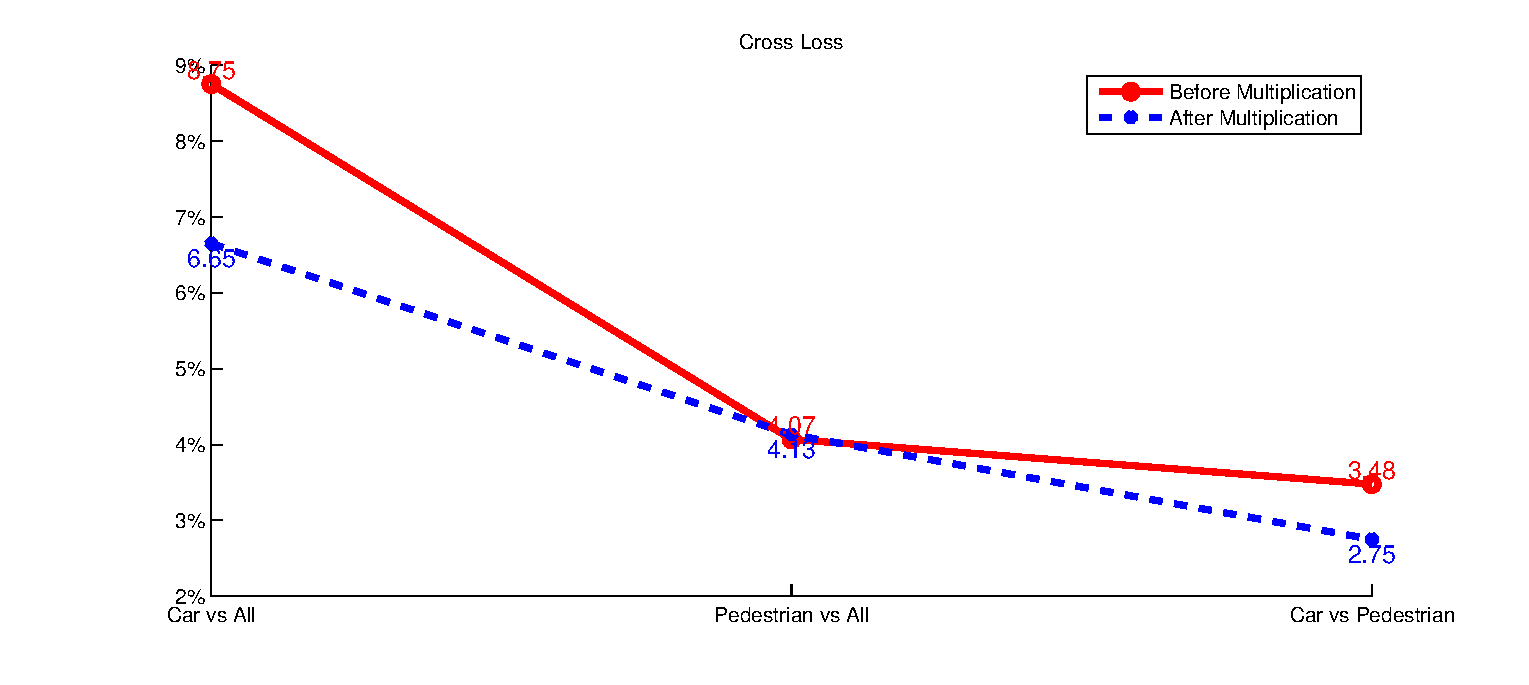
\includegraphics[width=\textwidth]{crossloss.eps}
%\fbox{\rule[-.5cm]{0cm}{4cm} \rule[-.5cm]{4cm}{0cm}}
\end{center}
\caption{Cross validation ($k=7$) loss before and after the image multiplication.
\label{fig:crossloss}}
\end{figure}

We can observe from Figure \ref{fig:crossloss} that the cross loss gets lower when we multiply the data set from $13908$ examples ($11288$ cars and $2620$ pedestrians) to $43536$ examples ($22576$ cars and $20960$ pedestrians). With this trick, we can make full use of the limited data set when we lack certain classes of objects. On the other hand, this trick also helps to balance the different light conditions among the images by adding random brightness bias. The final cross loss range from $2.75\%$ to $6.65\%$, which is satisfying. 

In addition to the randomly selected negative examples ($N_1=20000$), we add retrain step to enhance the training procedure. Though the number of positive examples is limited by the training set, we can crop much more negative examples from the existing images. But we need to balance that with the training cost. To be more effective, we save the false positive image segments to files during the validation, and add these images to the training set, labeled as the background image. These are considered to be the hard examples ($N_2=10500$), so finally we have $30500$ negative examples.

\subsubsection{Testing}

First we can test on the cropped testing set to evaluate the object recognition performance. Similarly, we can compare the different accuracy, precision, and recall rate we got before the image multiplication and after the image multiplication. We use the \texttt{predict} function from the MATLAB toolbox to classify with our trained SVM models.

\begin{figure}[htb]
\begin{center}
%\framebox[4.0in]{crossloss.eps}
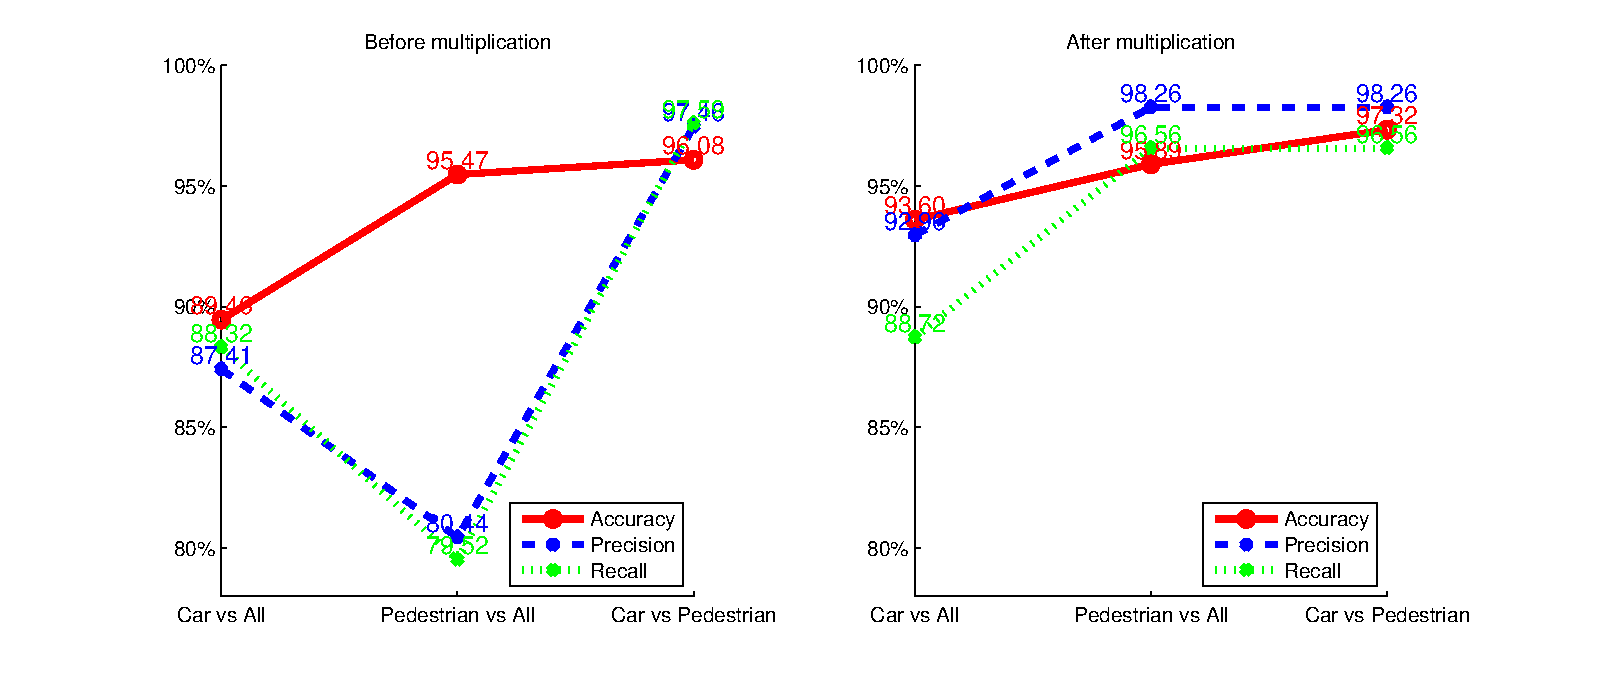
\includegraphics[width=\textwidth]{test_apr.eps}
%\fbox{\rule[-.5cm]{0cm}{4cm} \rule[-.5cm]{4cm}{0cm}}
\end{center}
\caption{Accuracy, precision, and recall rate before and after the image multiplication.
\label{fig:test_apr}}
\end{figure}

From Figure \ref{fig:test_apr}, we can conclude that multiplying images will also increase the accuracy, precision, and recall rate. Using $43536$ positive examples and $20000$ negative examples, we obtain a precision rate range from $92.96\%$ to $98.26\%$ and a recall rate range from $88.72\%$ to $96.56\%$. It is reasonable to consider that if we collect more training data or multiply more images with existing data, we will be able to get better performance. But that will also leads to more expensive training and testing cost. 

\subsection{CNN}

\section{Conclusion}



\iffalse
\begin{table}[htb]
\caption{title}
\label{sample-table}
\begin{center}
\begin{tabular}{ll}
\multicolumn{1}{c}{\bf PART}  &\multicolumn{1}{c}{\bf DESCRIPTION}
\\ \hline \\
Dendrite         &Input terminal \\
Axon             &Output terminal \\
Soma             &Cell body (contains cell nucleus) \\
\end{tabular}
\end{center}
\end{table}
\fi



\iffalse 

\sectinnnnnon{Submission of papers to NIPS 2015}

NIPS requires electronic submissions.  The electronic submission site is  
\begin{center}
   \url{http://papers.nips.cc}
\end{center}

Please read carefully the
instructions below, and follow them faithfully.
\subsection{Style}

Papers to be submitted to NIPS 2015 must be prepared according to the
instructions presented here. Papers may be only up to eight pages long,
including figures. Since 2009 an additional ninth page \textit{containing only
cited references} is allowed. Papers that exceed nine pages will not be
reviewed, or in any other way considered for presentation at the conference.
%This is a strict upper bound. 

Please note that this year we have introduced automatic line number generation
into the style file (for \LaTeXe and Word versions). This is to help reviewers
refer to specific lines of the paper when they make their comments. Please do
NOT refer to these line numbers in your paper as they will be removed from the
style file for the final version of accepted papers.

The margins in 2015 are the same as since 2007, which allow for $\approx 15\%$
more words in the paper compared to earlier years. We are also again using 
double-blind reviewing. Both of these require the use of new style files.

Authors are required to use the NIPS \LaTeX{} style files obtainable at the
NIPS website as indicated below. Please make sure you use the current files and
not previous versions. Tweaking the style files may be grounds for rejection.

%% \subsection{Double-blind reviewing}

%% This year we are doing double-blind reviewing: the reviewers will not know 
%% who the authors of the paper are. For submission, the NIPS style file will 
%% automatically anonymize the author list at the beginning of the paper.

%% Please write your paper in such a way to preserve anonymity. Refer to
%% previous work by the author(s) in the third person, rather than first
%% person. Do not provide Web links to supporting material at an identifiable
%% web site.

%%\subsection{Electronic submission}
%%
%% \textbf{THE SUBMISSION DEADLINE IS June 5, 2015. SUBMISSIONS MUST BE LOGGED BY
%% 23:00, June 5, 2015, UNIVERSAL TIME}

%% You must enter your submission in the electronic submission form available at
%% the NIPS website listed above. You will be asked to enter paper title, name of
%% all authors, keyword(s), and data about the contact
%% author (name, full address, telephone, fax, and email). You will need to
%% upload an electronic (postscript or pdf) version of your paper.

%% You can upload more than one version of your paper, until the
%% submission deadline. We strongly recommended uploading your paper in
%% advance of the deadline, so you can avoid last-minute server congestion.
%%
%% Note that your submission is only valid if you get an e-mail
%% confirmation from the server. If you do not get such an e-mail, please
%% try uploading again. 


\subsection{Retrieval of style files}

The style files for NIPS and other conference information are available on the World Wide Web at
\begin{center}
   \url{http://www.nips.cc/}
\end{center}
The file \verb+nips2015.pdf+ contains these 
instructions and illustrates the
various formatting requirements your NIPS paper must satisfy. \LaTeX{}
users can choose between two style files:
\verb+nips15submit_09.sty+ (to be used with \LaTeX{} version 2.09) and
\verb+nips15submit_e.sty+ (to be used with \LaTeX{}2e). The file
\verb+nips2015.tex+ may be used as a ``shell'' for writing your paper. All you
have to do is replace the author, title, abstract, and text of the paper with
your own. The file
\verb+nips2015.rtf+ is provided as a shell for MS Word users.

The formatting instructions contained in these style files are summarized in
sections \ref{gen_inst}, \ref{headings}, and \ref{others} below.

%% \subsection{Keywords for paper submission}
%% Your NIPS paper can be submitted with any of the following keywords (more than one keyword is possible for each paper):

%% \begin{verbatim}
%% Bioinformatics
%% Biological Vision
%% Brain Imaging and Brain Computer Interfacing
%% Clustering
%% Cognitive Science
%% Control and Reinforcement Learning
%% Dimensionality Reduction and Manifolds
%% Feature Selection
%% Gaussian Processes
%% Graphical Models
%% Hardware Technologies
%% Kernels
%% Learning Theory
%% Machine Vision
%% Margins and Boosting
%% Neural Networks
%% Neuroscience
%% Other Algorithms and Architectures
%% Other Applications
%% Semi-supervised Learning
%% Speech and Signal Processing
%% Text and Language Applications

%% \end{verbatim}

\section{General formatting instructions}
\label{gen_inst}

The text must be confined within a rectangle 5.5~inches (33~picas) wide and
9~inches (54~picas) long. The left margin is 1.5~inch (9~picas).
Use 10~point type with a vertical spacing of 11~points. Times New Roman is the
preferred typeface throughout. Paragraphs are separated by 1/2~line space,
with no indentation.

Paper title is 17~point, initial caps/lower case, bold, centered between
2~horizontal rules. Top rule is 4~points thick and bottom rule is 1~point
thick. Allow 1/4~inch space above and below title to rules. All pages should
start at 1~inch (6~picas) from the top of the page.

%The version of the paper submitted for review should have ``Anonymous Author(s)'' as the author of the paper.

For the final version, authors' names are
set in boldface, and each name is centered above the corresponding
address. The lead author's name is to be listed first (left-most), and
the co-authors' names (if different address) are set to follow. If
there is only one co-author, list both author and co-author side by side.

Please pay special attention to the instructions in section \ref{others}
regarding figures, tables, acknowledgments, and references.

\section{Headings: first level}
\label{headings}

First level headings are lower case (except for first word and proper nouns),
flush left, bold and in point size 12. One line space before the first level
heading and 1/2~line space after the first level heading.

\subsection{Headings: second level}

Second level headings are lower case (except for first word and proper nouns),
flush left, bold and in point size 10. One line space before the second level
heading and 1/2~line space after the second level heading.

\subsubsection{Headings: third level}

Third level headings are lower case (except for first word and proper nouns),
flush left, bold and in point size 10. One line space before the third level
heading and 1/2~line space after the third level heading.

\section{Citations, figures, tables, references}
\label{others}

These instructions apply to everyone, regardless of the formatter being used.

\subsection{Citations within the text}

Citations within the text should be numbered consecutively. The corresponding
number is to appear enclosed in square brackets, such as [1] or [2]-[5]. The
corresponding references are to be listed in the same order at the end of the
paper, in the \textbf{References} section. (Note: the standard
\textsc{Bib\TeX} style \texttt{unsrt} produces this.) As to the format of the
references themselves, any style is acceptable as long as it is used
consistently.

As submission is double blind, refer to your own published work in the 
third person. That is, use ``In the previous work of Jones et al.\ [4]'',
not ``In our previous work [4]''. If you cite your other papers that
are not widely available (e.g.\ a journal paper under review), use
anonymous author names in the citation, e.g.\ an author of the
form ``A.\ Anonymous''. 


\subsection{Footnotes}

Indicate footnotes with a number\footnote{Sample of the first footnote} in the
text. Place the footnotes at the bottom of the page on which they appear.
Precede the footnote with a horizontal rule of 2~inches
(12~picas).\footnote{Sample of the second footnote}

\subsection{Figures}

All artwork must be neat, clean, and legible. Lines should be dark
enough for purposes of reproduction; art work should not be
hand-drawn. The figure number and caption always appear after the
figure. Place one line space before the figure caption, and one line
space after the figure. The figure caption is lower case (except for
first word and proper nouns); figures are numbered consecutively.

Make sure the figure caption does not get separated from the figure.
Leave sufficient space to avoid splitting the figure and figure caption.

You may use color figures. 
However, it is best for the
figure captions and the paper body to make sense if the paper is printed
either in black/white or in color.
\begin{figure}[h]
\begin{center}
%\framebox[4.0in]{$\;$}
\fbox{\rule[-.5cm]{0cm}{4cm} \rule[-.5cm]{4cm}{0cm}}
\end{center}
\caption{Sample figure caption.}
\end{figure}

\subsection{Tables}

All tables must be centered, neat, clean and legible. Do not use hand-drawn
tables. The table number and title always appear before the table. See
Table~\ref{sample-table}.

Place one line space before the table title, one line space after the table
title, and one line space after the table. The table title must be lower case
(except for first word and proper nouns); tables are numbered consecutively.

\begin{table}[t]
\caption{Sample table title}
\label{sample-table}
\begin{center}
\begin{tabular}{ll}
\multicolumn{1}{c}{\bf PART}  &\multicolumn{1}{c}{\bf DESCRIPTION}
\\ \hline \\
Dendrite         &Input terminal \\
Axon             &Output terminal \\
Soma             &Cell body (contains cell nucleus) \\
\end{tabular}
\end{center}
\end{table}

\section{Final instructions}
Do not change any aspects of the formatting parameters in the style files.
In particular, do not modify the width or length of the rectangle the text
should fit into, and do not change font sizes (except perhaps in the
\textbf{References} section; see below). Please note that pages should be
numbered.

\section{Preparing PostScript or PDF files}

Please prepare PostScript or PDF files with paper size ``US Letter'', and
not, for example, ``A4''. The -t
letter option on dvips will produce US Letter files.

Fonts were the main cause of problems in the past years. Your PDF file must
only contain Type 1 or Embedded TrueType fonts. Here are a few instructions
to achieve this.

\begin{itemize}

\item You can check which fonts a PDF files uses.  In Acrobat Reader,
select the menu Files$>$Document Properties$>$Fonts and select Show All Fonts. You can
also use the program \verb+pdffonts+ which comes with \verb+xpdf+ and is
available out-of-the-box on most Linux machines.

\item The IEEE has recommendations for generating PDF files whose fonts
are also acceptable for NIPS. Please see
\url{http://www.emfield.org/icuwb2010/downloads/IEEE-PDF-SpecV32.pdf}

\item LaTeX users:

\begin{itemize}

\item Consider directly generating PDF files using \verb+pdflatex+
(especially if you are a MiKTeX user). 
PDF figures must be substituted for EPS figures, however.

\item Otherwise, please generate your PostScript and PDF files with the following commands:
\begin{verbatim} 
dvips mypaper.dvi -t letter -Ppdf -G0 -o mypaper.ps
ps2pdf mypaper.ps mypaper.pdf
\end{verbatim}

Check that the PDF files only contains Type 1 fonts. 
%For the final version, please send us both the Postscript file and
%the PDF file. 

\item xfig "patterned" shapes are implemented with 
bitmap fonts.  Use "solid" shapes instead. 
\item The \verb+\bbold+ package almost always uses bitmap
fonts.  You can try the equivalent AMS Fonts with command
\begin{verbatim}
\usepackage[psamsfonts]{amssymb}
\end{verbatim}
 or use the following workaround for reals, natural and complex: 
\begin{verbatim}
\newcommand{\RR}{I\!\!R} %real numbers
\newcommand{\Nat}{I\!\!N} %natural numbers 
\newcommand{\CC}{I\!\!\!\!C} %complex numbers
\end{verbatim}

\item Sometimes the problematic fonts are used in figures
included in LaTeX files. The ghostscript program \verb+eps2eps+ is the simplest
way to clean such figures. For black and white figures, slightly better
results can be achieved with program \verb+potrace+.
\end{itemize}
\item MSWord and Windows users (via PDF file):
\begin{itemize}
\item Install the Microsoft Save as PDF Office 2007 Add-in from
\url{http://www.microsoft.com/downloads/details.aspx?displaylang=en\&familyid=4d951911-3e7e-4ae6-b059-a2e79ed87041}
\item Select ``Save or Publish to PDF'' from the Office or File menu
\end{itemize}
\item MSWord and Mac OS X users (via PDF file):
\begin{itemize}
\item From the print menu, click the PDF drop-down box, and select ``Save
as PDF...''
\end{itemize}
\item MSWord and Windows users (via PS file):
\begin{itemize}
\item To create a new printer
on your computer, install the AdobePS printer driver and the Adobe Distiller PPD file from
\url{http://www.adobe.com/support/downloads/detail.jsp?ftpID=204} {\it Note:} You must reboot your PC after installing the
AdobePS driver for it to take effect.
\item To produce the ps file, select ``Print'' from the MS app, choose
the installed AdobePS printer, click on ``Properties'', click on ``Advanced.''
\item Set ``TrueType Font'' to be ``Download as Softfont''
\item Open the ``PostScript Options'' folder
\item Select ``PostScript Output Option'' to be ``Optimize for Portability''
\item Select ``TrueType Font Download Option'' to be ``Outline''
\item Select ``Send PostScript Error Handler'' to be ``No''
\item Click ``OK'' three times, print your file.
\item Now, use Adobe Acrobat Distiller or ps2pdf to create a PDF file from
the PS file. In Acrobat, check the option ``Embed all fonts'' if
applicable.
\end{itemize}

\end{itemize}
If your file contains Type 3 fonts or non embedded TrueType fonts, we will
ask you to fix it. 

\subsection{Margins in LaTeX}
 
Most of the margin problems come from figures positioned by hand using
\verb+\special+ or other commands. We suggest using the command
\verb+\includegraphics+
from the graphicx package. Always specify the figure width as a multiple of
the line width as in the example below using .eps graphics
\begin{verbatim}
   \usepackage[dvips]{graphicx} ... 
   \includegraphics[width=0.8\linewidth]{myfile.eps} 
\end{verbatim}
or % Apr 2009 addition
\begin{verbatim}
   \usepackage[pdftex]{graphicx} ... 
   \includegraphics[width=0.8\linewidth]{myfile.pdf} 
\end{verbatim}
for .pdf graphics. 
See section 4.4 in the graphics bundle documentation (\url{http://www.ctan.org/tex-archive/macros/latex/required/graphics/grfguide.ps}) 
 
A number of width problems arise when LaTeX cannot properly hyphenate a
line. Please give LaTeX hyphenation hints using the \verb+\-+ command.


\subsubsection*{Acknowledgments}

Use unnumbered third level headings for the acknowledgments. All
acknowledgments go at the end of the paper. Do not include 
acknowledgments in the anonymized submission, only in the 
final paper. 

\fi 

\bibliographystyle{IEEEtran}
\bibliography{ref}


\subsubsection*{Old References}

\iffalse
References follow the acknowledgments. Use unnumbered third level heading for
the references. Any choice of citation style is acceptable as long as you are
consistent. It is permissible to reduce the font size to `small' (9-point) 
when listing the references. {\bf Remember that this year you can use
a ninth page as long as it contains \emph{only} cited references.}
\fi 

\small{

[1] C. G. Keller, M. Enzweiler, and D. M. Gavrila, “A new benchmark for stereo-based pedestrian detection,” in 2011 IEEE Intelligent Vehicles Symposium (IV), 2011, pp. 691–696.

[2] A. Geiger, P. Lenz, and R. Urtasun, “Are we ready for autonomous driving? The KITTI vision benchmark suite,” in 2012 IEEE Conference on Computer Vision and Pattern Recognition, 2012, pp. 3354–3361.

[3] Y. Tian, P. Luo, X. Wang, and X. Tang, “Deep Learning Strong Parts for Pedestrian Detection,” in 2015 IEEE International Conference on Computer Vision, 2015.

[4] L. Huang, Y. Yang, Y. Deng, and Y. Yu, “DenseBox: Unifying Landmark Localization with End to End Object Detection,” arXiv:1509.04874, 2015.

[5] J. Long, E. Shelhamer, and T. Darrell, “Fully convolutional networks for semantic segmentation,” arXiv1411.4038, 2014.

[6] A. Krizhevsky, I. Sutskever, and G. Hinton, “Imagenet classification with deep convolutional neural networks,” Adv. Neural Inf. Process. Syst. 25, 2012.

[7] P. Dollar, C. Wojek, B. Schiele, and P. Perona, “Pedestrian detection: A benchmark,” in 2009 IEEE Conference on Computer Vision and Pattern Recognition, 2009, pp. 304–311.

[8] K. Sande, J. Uijlings, T. Gevers, and A. Smeulders, Segmentation as Selective Search for Object Recognition, in 2011 IEEE International Conference on Computer Vision, pp. 1879-1886.
%Other paper

\iffalse
[1] Alexander, J.A. \& Mozer, M.C. (1995) Template-based algorithms
for connectionist rule extraction. In G. Tesauro, D. S. Touretzky
and T.K. Leen (eds.), {\it Advances in Neural Information Processing
Systems 7}, pp. 609-616. Cambridge, MA: MIT Press.

[2] Bower, J.M. \& Beeman, D. (1995) {\it The Book of GENESIS: Exploring
Realistic Neural Models with the GEneral NEural SImulation System.}
New York: TELOS/Springer-Verlag.

[3] Hasselmo, M.E., Schnell, E. \& Barkai, E. (1995) Dynamics of learning
and recall at excitatory recurrent synapses and cholinergic modulation
in rat hippocampal region CA3. {\it Journal of Neuroscience}
{\bf 15}(7):5249-5262.
}
\fi

\end{document}
